%\documentclass{recpad2k}
\documentclass[extendedabs]{recpad2k}
\usepackage[acronym]{glossaries}
\usepackage{lipsum}
\usepackage{multicol}
\usepackage{multirow} 
\usepackage{booktabs}
\usepackage{float}
\bibliographystyle{unsrtnat}

%% Enter your paper number here for the review copy
\recpadreviewcopy{??}

\title{Impact of Interference on Time-Of-Flight LiDAR}

% Enter the paper's authors in order
% \addauthor{Name}{email/homepage}{INSTITUTION_CODE}
\addauthor{Pedro Martins}{martinspedro@ua.pt}{1}
\addauthor{Ant\'onio Neves}{an@ua.pt}{1}
\addauthor{Miguel Drummond}{mvd@av.it.pt}{2}
\addauthor{Andr\'e Albuquerque}{Andre.Albuquerque@pt.bosch.com}{3}

% Enter the institutions
% \addinstitution{Name\\Address}
\addinstitution{
 University of Aveiro\\
 Campus Universit\'ario de Santiago\\
 Dpt. Electronics, Telecommunications and Informatics 
 Aveiro, Portugal
}
\addinstitution{
 Instituto de Telecomunica\c{c}\~oes\\
 Campus Universit\'ario de Santiago,\\
 Aveiro, Portugal
}
\addinstitution{
Bosch Car Multim\'edia Portugal, S.A \\
 Braga, Portugal
}

\runninghead{Student, Prof, Prof, Collaborator}{RECPAD Author Guidelines}

% Any macro definitions you would like to include
% These are not defined in the style file, because they don't begin
% with \bmva, so they might conflict with the user's own macros.
% The \bmvaOneDot macro adds a full stop unless there is one in the
% text already.
\def\eg{\emph{e.g}\bmvaOneDot}
\def\Eg{\emph{E.g}\bmvaOneDot}
\def\etal{\emph{et al}\bmvaOneDot}

\newcommand{\me}{\mathrm{e}}
%------------------------------------------------------------------------- 
% Document starts here
\begin{document}


\maketitle

% Acronyms List
\newacronym{lidar}{LiDAR}{Light Detection And Ranging}
\newacronym{tof}{TOF}{Time of Flight}
\newacronym{adas}{ADAS}{Advanced Driver-Assistance Systems}
\newacronym{ros}{ROS}{Robotic Operative System}
\newacronym{pcl}{PCL}{Point Cloud Library}
\newacronym{slam}{SLAM}{Simultaneous Location and Mapping}
\newacronym{msl}{MSL}{Middle Size League}
\newacronym{icp}{ICP}{Iterative Closest Point}
\newacronym{rpm}{RPM}{Rotations Per Minute}


\begin{abstract}
A research on the interference between \gls{lidar} was conducted. The main objective is to assess its impact and behavior, since most of the self-driving vehicles rely on \gls{lidar} technology for navigation. Two conditions were studied: the distance between the \gls{lidar}s and the length of the voxel grid edges used for the statistical analysis. Our findings indicate that a smaller length of the voxel grid edges increases slightly the magnitude of the interference, for a fixed distance. Regarding the distance, no conclusion is possible, since other factor appear to be more relevant. In a worst case scenario, we conclude that one in each thousand points is expected to be interfered when two \gls{lidar}s coexist.
\end{abstract}

%------------------------------------------------------------------------- 
\section{Introduction}
\label{sec:intro}

%Since the appearance of \gls{adas}, consumers, experts and governments hoped that ``smarter'' cars would result in safer roads. 
Backed both by common sense and research, human error is still one of the causes of most accidents and injuries on the road \cite{Bimbraw2015, world2019global}. Despite increasingly road safety awareness campaigns, laws and heavier fines, annual global road traffic deaths have reached 1.35 million in 2018, being the leading cause of death for people aged 5-29 years \cite{world2019global}.

Several studies have been conducted on self-driving technology and \Gls{adas} \cite{Fridman2017, ADAS1, Bimbraw2015}, which appears has one of the most promising solutions to mitigate road accidents. Along with some public datasets that have been made available to further the development of self-driving vehicles \cite{Geiger2012}, \gls{adas} is becoming more relevant, mainly due to the maturation of \gls{lidar} technology \cite{Sullivan2016}. 

\gls{lidar} sensors map their surroundings thanks to their capability of precisely measure depth - with a few centimeters of error, over distances that can range until 100 meters \cite{vlp16, Sullivan2016}. \gls{tof} \gls{lidar}, the most common type, acquires depth information by measuring the time elapsed between the emission and reception of a laser pulse reflected from a surrounding target \cite{Sullivan2016}. To scan a single line, a single pair of laser and photodetector are assembled on a rotational device, creating a 2D \gls{lidar}. If multiple pairs are assembled together, on a rotational device, with different polar angles, the \gls{lidar} is said to be a 3D \gls{lidar}.

These maps, commonly represented as point clouds or mesh clouds, are one of the preferred method for \gls{slam} algorithms, which allow a vehicle without previous knowledge of its surroundings to autonomous navigate them - a crucial task for \gls{adas} on self-driving vehicles.

%Normally, this pair of laser and photodetector is assembled on a rotational device, allowing a single pair to measure a line, creating a 2D \gls{lidar}. If multiple pairs are assembled together, with different polar angles, the \gls{lidar} is said to be 3D, since a total revolution can produce a three dimensional map of its surroundings. 





%However, despite being a complex and broad research area, most of the current state-of-the-art for autonomous driving relies heavily on \gls{lidar} - a device capable of measuring the depth from a scene by using laser beams. 

%\subsection{\gls{lidar}}
 

%The most common \gls{lidar} sensor is a 

%Combining the reliability of the depth measurement with the assemblage of multiple pairs of laser and photodetectors on a fast rotational device (typically 5 to 20 Hz) creates one of the most appealing and reliable sensors for self-driving vehicles and \gls{adas}.

\subsection{\gls{lidar} Interference}
\gls{tof} \gls{lidar}s basic principle implies that when a laser pulse is emitted, three different scenarios are possible, being the first one the only one that produces a valid measurement:
\begin{enumerate}
    \itemsep0em
    \item The laser pulse returns, due to the reflection of an obstacle;
    \item The laser pulse does not return;
    \item The laser pulse returns with intensity below the noise floor.
\end{enumerate}

Interference and crosstalk between the pairs of laser and photodetectors on a \gls{lidar} are mitigated with different firing offsets, or in the case of mutual interference between \gls{lidar}, it is possible to synchronize their firing time using specialized clock signals \cite{vlp16}.

However, in a society when self-driving vehicles coexist, another scenario is possible: a \gls{lidar} ``A'' fires a laser pulse that is received, directly or indirectly, by the photodetector on a \gls{lidar} ``B''. Since \gls{lidar} ``B'' measures the distance to an obstacle by measuring the time between the firing and reception of its own laser pulse, the reception of another laser pulse causes an erroneous measure with an unpredictable behavior. If this interference is significant, the reliability of the \gls{lidar} and consequently autonomous vehicles and \gls{adas} is seriously undermined, due to the incapability to accurately mapping their surroundings.

To the best of the author' knowledge, despite the relevance of the topic to a society of self-driving cars, there are only available the studies conducted by Kim \etal \cite{Kim2017, Kim2015}, which seek to characterize this interference; and by Retterath and Laumeyer \cite{Al.2013}, seeking to provide an apparatus for reducing the mutual interference of \gls{lidar} sensors on the same vehicle.

%Despite the relevance of the topic for the massification of self-driving vehicles and the hazardous impact on \Gls{adas} reliability, the research topic presented in this paper has received very reduced attention by the research community. 
%A major \gls{lidar} manufacture also addresses the problem of mutual interference of the \gls{lidar} sensors on the same vehicle, by allowing their synchronization and laser firing in different instants \cite{vlp16}.

Kim \etal research %despite using a 2D \gls{lidar}%instead of a 3D \gls{lidar}
is the only study to use two independent 2D \gls{lidar}s interfering with each other. Kim \etal results indicate that interference has spatial and temporal locality \cite{Kim2015} and in any given time, in Kim's setup, a data point has 0.05 \% probability of being interfered \cite{Kim2015}.
%The former states that if a particular angle is interfered, the following angles are likely to also be interfered; while the latter indicates that if a measure is interfered, on the following frame that same measure is also likely to be interfered. 
%However, 


\subsection{Proposed Work}
This research intends to understand the impact of the interference between 3D \gls{lidar}, whose reliability is crucial for self-driving vehicles, consequently expanding Kim's research.
Our proposal consists on assessing the interference behavior with the relative distance between \gls{lidar}s and the length of the voxel\footnote{A voxel is an element of a 3D grid that is equally spaced, representing a single point.} grid used to quantify this interference.

This paper is organized as follows. Section 1 presents the introduction and motivation for this work. Section 2 debates the related work. The third section shows the experimental results obtained. Section 4 contains the method developed for interference analysis. The results and their discussion is presented on Section 5. Section 6 deliberates on the paper's conclusions.


%\section{Related Work}
%\label{sec:related_work}

%To the best of the author' knowledge, despite the relevance of the topic to a society of self-driving cars, there are only available the studies conducted by Kim \etal \cite{Kim2017, Kim2015}, which seek to characterize this interference; and by Retterath and Laumeyer \cite{Al.2013}, seeking to provide an apparatus for reducing the mutual interference of \gls{lidar} sensors on the same vehicle.

%Despite the relevance of the topic for the massification of self-driving vehicles and the hazardous impact on \Gls{adas} reliability, the research topic presented in this paper has received very reduced attention by the research community. 
%A major \gls{lidar} manufacture also addresses the problem of mutual interference of the \gls{lidar} sensors on the same vehicle, by allowing their synchronization and laser firing in different instants \cite{vlp16}.

%Kim \etal research, despite using a 2D \gls{lidar} instead of a 3D \gls{lidar}, is the only study to use two independent \gls{lidar}s interfering with each other. Kim \etal results indicate that interference has spatial and temporal locality. The former states that if a particular angle is interfered, the following angles are likely to also be interfered; while the latter indicates that if a measure is interfered, on the following frame that same measure is also likely to be interfered. However, in any given time, in Kim's setup, a data point has 0.05 \% probability of being interfered \cite{Kim2015}.



\section{Experimental Setup}
\label{sec:experimental_setup}
To analize the impact of \gls{lidar} interference, two \gls{lidar}s were used. One acts as the source \gls{lidar}, which acquires data from its surroundings and the other acts as an interference generator on the data acquired by the first.  
The source \gls{lidar} is a Velodyne VLP-16, which contains 16 laser beams and is fixed on the table. The \gls{lidar} acting as an interference generator is a Hesai Pandar40, which has 40 lasers, and is fixed on a tripod. Both \gls{lidar}s rotate at 600 \gls{rpm}.

%Datasets were acquired under different interference scenarios, by varying the distance, height and relative direction between both \gls{lidar}s and by blocking their direct interference while varying their distance.

To capture, manage and analyze the datasets, software was developed in C++, using the \gls{ros} framework and the \gls{pcl}. \gls{ros} was also used for the interaction with the sensors and to allow near real-time operation on a standard laptop computer.

Figure \ref{fig:experimental_setup} shows a picture of the described setup on one of the test scenarios, a robotic \gls{msl} soccer field.

\begin{figure}[h]
    \centering
    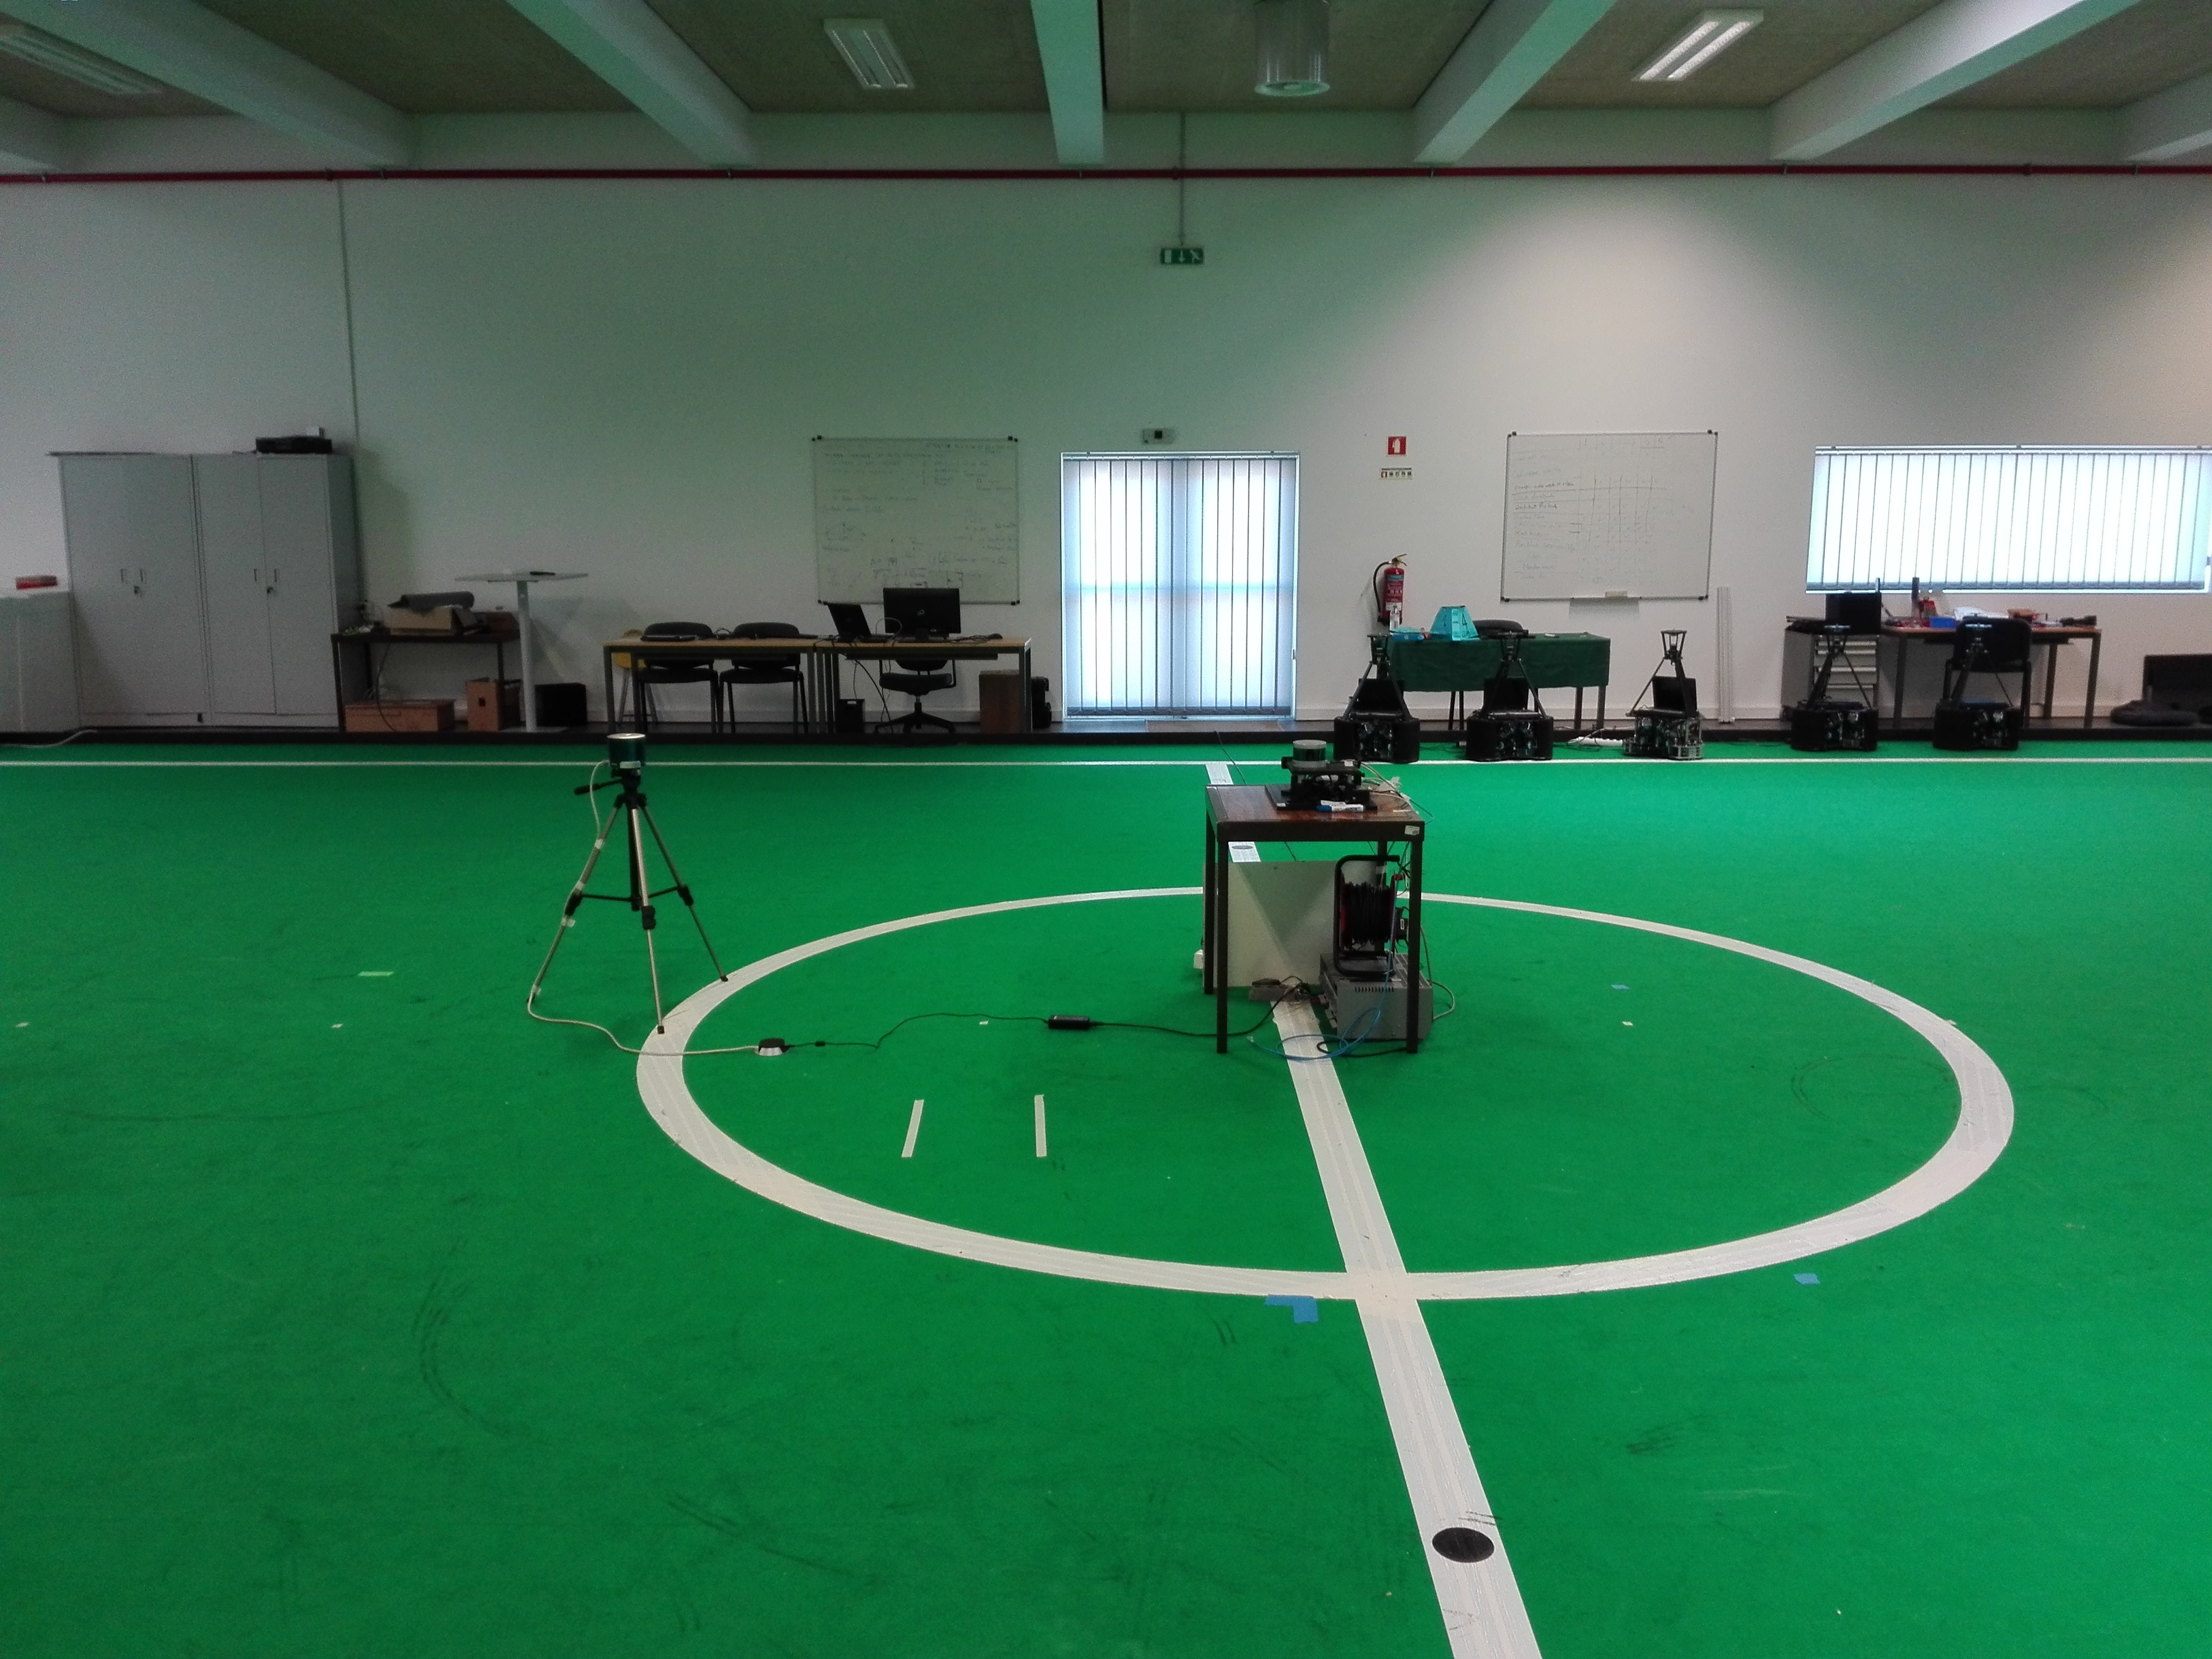
\includegraphics[width=0.45\textwidth]{images/CAMBADA_experimenta_setup.jpg}
    \caption{Experimental setup described on section \ref{sec:experimental_setup}, used for the data presented on this research.}
    \label{fig:experimental_setup}
\end{figure}

\section{Methodology}
\label{sec:methodology}
Since it is not possible to distinguish an interfered from a valid measure (from an hardware standpoint, both of them are valid measures), we propose a method to distinguish which measures result from \gls{lidar} interference.

The proposed method assumes a static scenario and compares the point clouds with and without interference. First, the \gls{lidar}s are positioned and the interference generator \gls{lidar} is off. On these conditions, several point clouds are recorded and merged to create a ground truth model. Then, the \gls{lidar} that causes the interference is switched on and several point clouds are registered.

The first data acquisition is used to generate the ground truth model of the scenario, free from interference, by stitching together the different frames using the \gls{icp} algorithm. A voxel grid filter is also applied to every frame, to filter out noisy points, reduce the number of points and ensure more uniform point density.

%\subsection{Ground Truth Generation}
%The ground truth model generation is an iterative process that stitches together every point cloud generated recorded, improving the ground truth model. First, a Voxel Grid Filter is applied to filter out redundant points from the point cloud to be merged. Secondly, an \gls{icp} algorithm finds the transform that aligns the two clouds. Lastly, the clouds are aligned and a voxel filter is applied again to the resulting cloud.

%A voxel filter is point cloud technique that divides the space in cubes of a defined dimension. For every cube, the centroid of all the points contained within the cube are computed and considered as an approximation of all the points.

%This technique ensures that noisy points are filtered out from the scenario ground truth model, the model has a more uniform point density and that the number of points is reduced.


%\subsection{Interference Analysis}
To quantify the interference, each point cloud containing interference is compared with the ground truth model.
The occurrence of interference is measured relatively to the total number of voxels and represents the number of modified voxels (i.e., the number of voxels who were occupied and were freed and vice-versa) when comparing the ground truth model with the point cloud containing interference.

%The comparison algorithm is based on the detection of change in voxels (occupied vs non-occupied and vice-versa). 

%The point cloud data is used to initialize an octree - a data structure used to efficiently store 3D data. Then, the octree resulting from each interfered point cloud is individually compared with the octree resulting from the ground truth model.

%To quantify the degree of interference, a change detection algorithm is applied to measure the number of voxels modified between the two octrees. By knowing the total number of voxels, it is possible to determine how much voxels have been interfered and provide a statisfical figure on the severity of the mutual \gls{lidar} interference.

\section{Results}
For a fixed \gls{lidar} height, direction and rotation speed, both \gls{lidar}s optical center were aligned and several point clouds were recorded while the interference generator \gls{lidar} was active. Using the method described in Section \ref{sec:methodology}, the quotient of interfered vs total number of voxels was calculated for a relative distance varying meter by meter from 1 to 12 m and considering voxel edge lengths ranging from 10 to 50 centimeters, with steps of 10 cm. The results are presented on figure \ref{fig:results}, on the form of a contour graph. 

The smaller the voxel edge length (horizontal axis), the higher the number of voxels per point cloud. Analyzing figure \ref{fig:results} concludes that the number of voxels affected by interference increases with the decrease of the voxel edge length. If a fixed voxel edge length is considered, one can noticed that the results are more prone to variations with the distance, being this variation more significantly at smaller voxel edge lengths.


These results lead us to believe that despite the variation with the distance between the \gls{lidar}, there are other factors that drastically influence the interference. Such analysis is yet to be conducted and it is left for future work.

The experimental results also show that on the worst case scenario, in every 1000 measurements there is an interfered measure (27 points per frame that correspond to 270 points per second). The best case scenario is 1 interfered point for every 100000 points, which is less than a point per second.

\begin{figure}
    \centering
    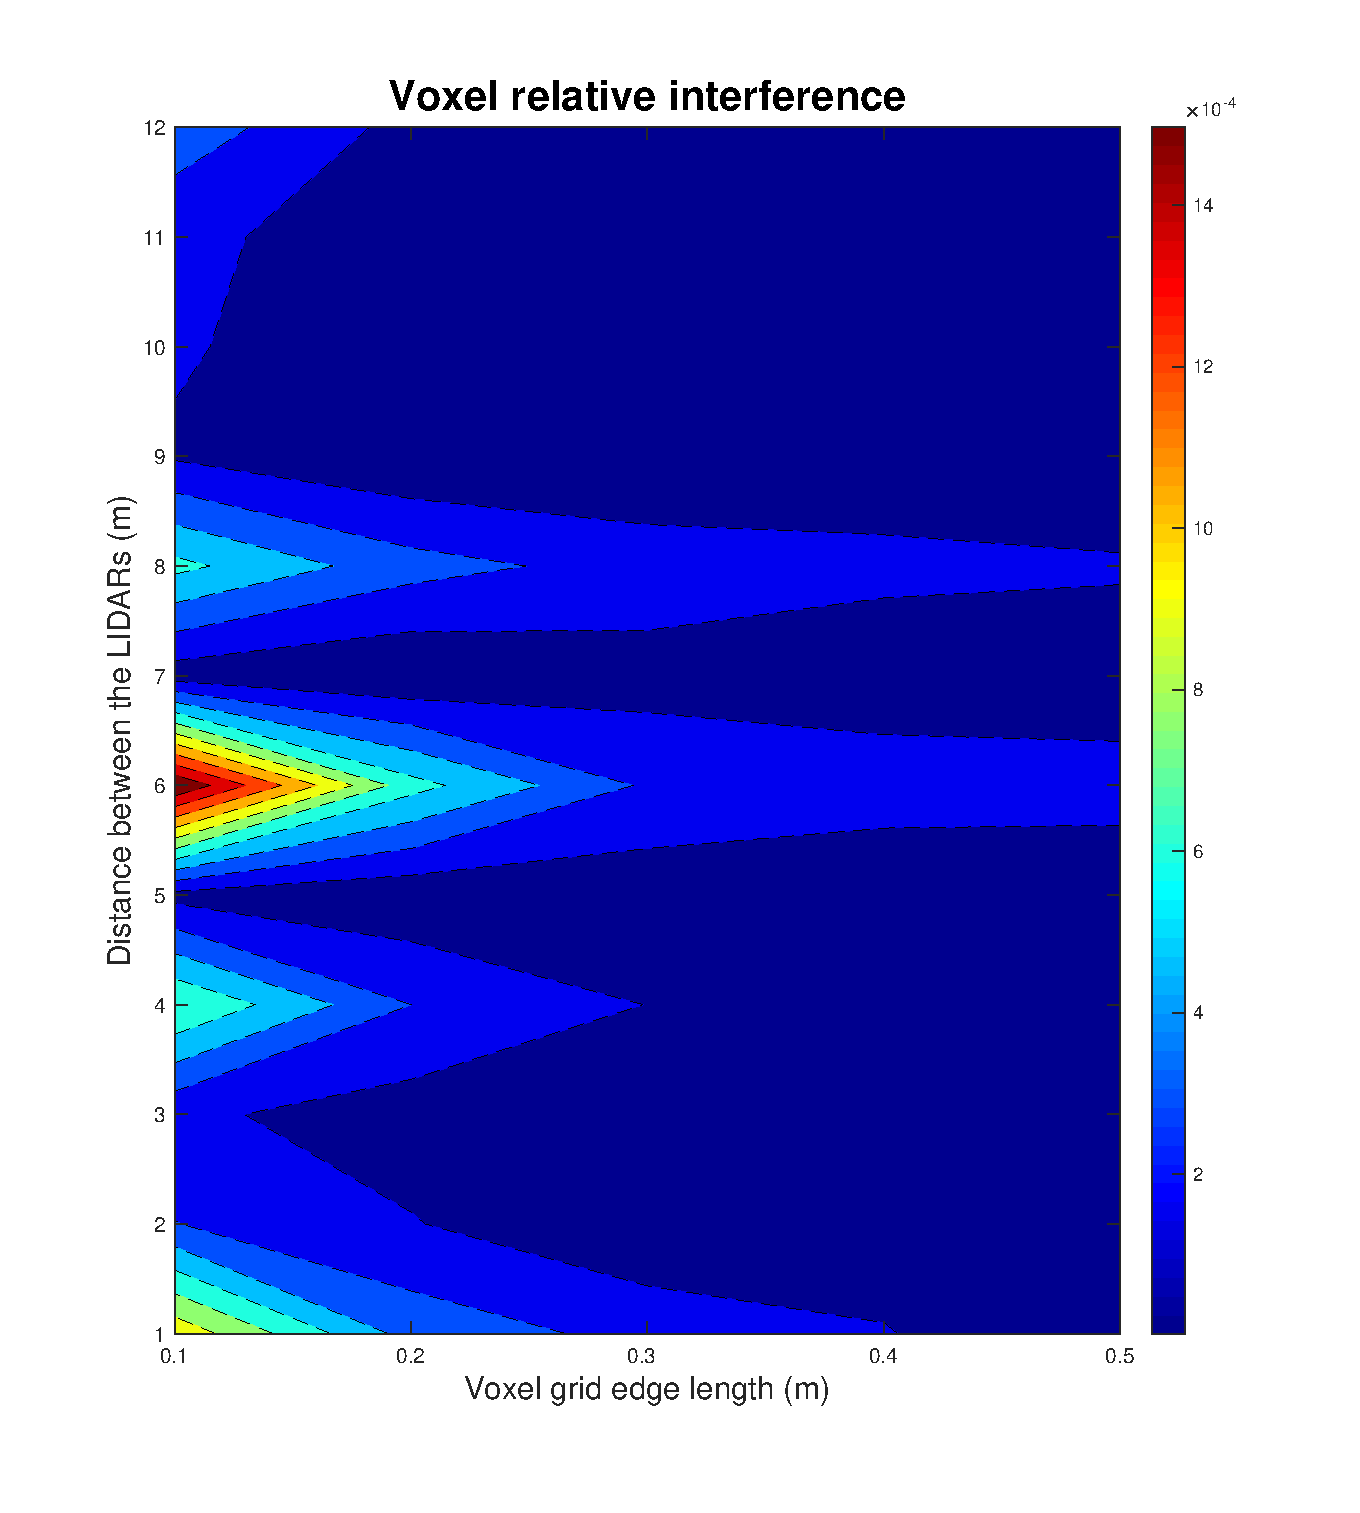
\includegraphics[width=0.45\textwidth]{images/contour.eps}
    \caption{Contour graph of the results. On the horizontal axis the voxel edge length is varied between 0.1 and 0.5 m with steps of 0.1 m. On the vertical axis, the relative distance (keeping the \gls{lidar} orientation with zero azimutal angle) is varied meter by meter between 1 and 12 meters.}
    \label{fig:results}
\end{figure}

\section{Conclusion}
Interference between \gls{tof} \gls{lidar} is a research topic that is yet to receive the attention of the academic community, due to its impact on self-driving vehicles. The extensive adoption and reliance on \gls{lidar} technology for self-driving vehicles will force the coexistent of these laser sensors on real world scenarios, which, by our findings, will resulting on mutual interference between \gls{lidar}s, causing errors on the measured data.

On this article, a study of the interference between \gls{tof} \gls{lidar}s is conducted. Previous available results have shown that on 2D \gls{lidar}s an error of 1 in 10000 points is expected \cite{Kim2017, Kim2015}. Our findings not only extended this study to 3D \gls{lidar}s, more common in self-driving vehicles, but also discovered that the severity of errors is highly volatile and can be one order of magnitude higher than previous findings.

Analysis were performed by varying the distance between the \gls{lidar}s and by changing the voxel grid edge size. We conclude that the lower the voxel grid edge length, the higher the effects of the interference. Increasing the distance between the \gls{lidar} resulted on a behaviour that has no obvious correlation with the distance. Therefore further investigations are required to identify the main factors influencing mutual interference between \gls{lidar}s and to quantify their severity in object detection and recognition.


%------------------------------------------------------------------------- 
\footnotesize
\bibliography{egbib}
\end{document}
